\begin{frame}{Facets on Pt nanoparticles}
    \begin{columns}
        \column[T]{0.45\textwidth}
        \centering
        A: $\diameter \approx 800 nm$ 
        \begin{figure}
            \centering
            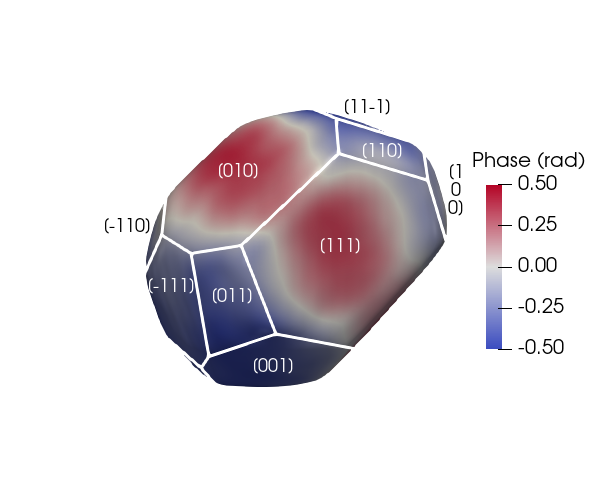
\includegraphics[trim=50 50 130 100, clip, width=\textwidth]{Figures/bcdi_data/D6/D6_facets.png}
            \label{fig:facets_D6}
        \end{figure}

        \column[T]{0.55\textwidth}
        \centering
        B: $\diameter \approx 350 nm$ 

        \begin{figure}
            \centering
            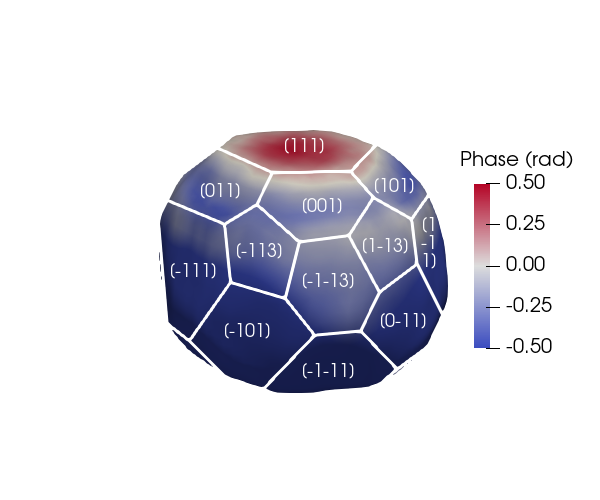
\includegraphics[trim=50 50 0 100, clip, width=\textwidth]{Figures/bcdi_data/B7/B7_facets.png}
            \label{fig:facets_B7}
        \end{figure}

    \end{columns}

    \pause
    \centering
    \vspace{-1em}
    \begin{itemize}
        \item \textcolor{Important}{Difference in size, shape, and in the type of facets exhibited.}
        \pause
        \item Most of the facets have low miller indices, (100), (110), (111).
        \pause
        \item The smaller nanoparticle has more 'open' facets such as Pt (311)
        \pause
        \item The area between different facets in considered to be edges or corners, depending on the coordination geometry.
    \end{itemize}
    
\end{frame}